\subsection{Dane wejściowe}

    \begin{enumerate}
        \item 
            \begin{flushleft}
                Parametry cieczy schładzanej
                \begin{itemize}
                    \item Toluen
                    \item Temperatura wejściowa \(T_{1we} = 75\DEGc\)
                    \item Temperatura wyjściowa \(T_{1wy} = 55\DEGc\)
                    \item Strumień masy    \(m_{1} = 3\FLOWRATEkgs\)
                    \item Dodatkowe parametry czynnika dla \(T=T_{1średnie}=\frac{T_{1we}+T_{1wy}}{2}=65\DEGc\)
                        \begin{figure}[h]
                            \centering
                            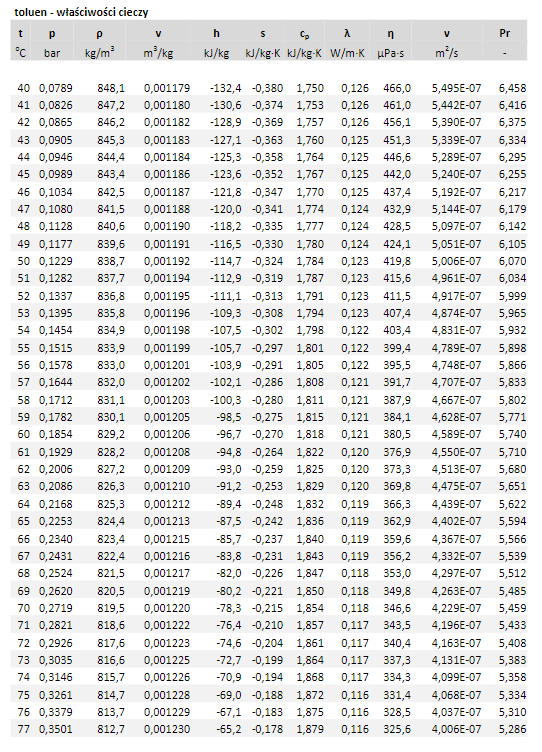
\includegraphics[width=\linewidth-130px]{Tabela_toluen.PNG}
                        \end{figure}
                \end{itemize}
            \end{flushleft} 
        \pagebreak
        \item 
            \begin{flushleft}
                Parametry cieczy chłodzącej
                \begin{itemize}
                    \item Woda
                    \item Temperatura wejściowa \(T_{2we} = 10\DEGc\)
                    \item Temperatura wyjściowa \(T_{2wy} = 30\DEGc\)
                    \item Prędkość przepływu    \(U_{1} = 0.1-1\VELOCITY\)
                    \item Dodatkowe parametry czynnika \item Dodatkowe parametry czynnika dla \(T=T_{2średnie}=\frac{T_{2we}+T_{2wy}}{2}=20\DEGc\)
                        \begin{figure}[h]
                            \centering
                            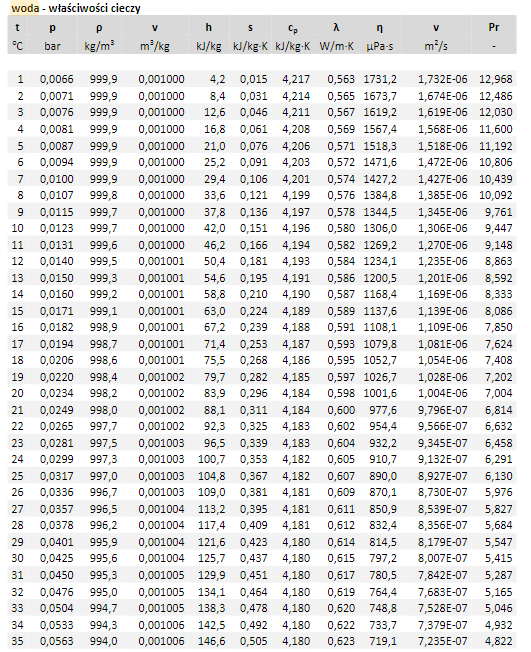
\includegraphics[width=\linewidth-130px]{Tabela_woda.PNG}
                        \end{figure}
                    \end{itemize}
            \end{flushleft}
        \pagebreak    
    \end{enumerate}
    

